\newcommand\emmax[1]{\textcolor{red}{\textbf{#1}}}
\newcommand\methodyear[1]{\textcolor{blue}{#1}}
\newcommand\Tstrut{\rule{0pt}{2.6ex}}
\newcommand\Bstrut{\rule[-0.9ex]{0pt}{0pt}}

% Please add the following required packages to your document preamble:
% \usepackage{multirow}

\newcommand\iw{0.0}
\newcommand\cw{0.05}

\begin{table*}[!htb]
    \renewcommand{\arraystretch}{1.2}
    \caption{Accuracy(\%) of each method with 10 shared class on Office-31. }
    \label{table: exp on office31}

    \centering
    \small
    \begin{tabularx}{0.95\textwidth}{r Y@{\hskip \iw in}Y Y@{\hskip \iw in}Y Y@{\hskip \iw in}Y Y@{\hskip \iw in}Y Y@{\hskip \iw in}Y Y@{\hskip \iw in}Y >{\itshape}Y@{\hskip \iw in}>{\itshape}Y}
    % \begin{tabularx}{0.95\textwidth}{r XX XX XX XX XX XX >{\itshape}Y>{\itshape}Y}
        \toprule[0.8pt]
        \multicolumn{1}{c}{\multirow{2}{*}{Method}} & \multicolumn{14}{c}{All Class Accuracy(\textbf{OS}) and Known Class Accuracy(\textbf{OS*}) on Office31}                                                                                                                                                                                                                                                                                                                           \\ \cmidrule[0.1pt]{2-15}

        \multicolumn{1}{c}{}                        & \multicolumn{2}{c}{A $\to$ D}                                 & \multicolumn{2}{c}{A $\to$ W} & \multicolumn{2}{c}{D $\to$ A} & \multicolumn{2}{c}{D $\to$ W} & \multicolumn{2}{c}{W $\to$ A} & \multicolumn{2}{c}{W $\to$ D} & \multicolumn{2}{c}{\textit{AVG}}                                                                                                                                  \\
        \hline
        \multicolumn{15}{c}{\textit{results in CSDA setting}}  \\
        \hline
        GRL \methodyear{[JMLR, 2016]} &-& 91.3&-& 91.8&-& 90.1&-& 98.6&-& 89.6&-& 99.7&-&93.5\\
        MMD \methodyear{[NIPS, 2007]} &-& 90.3&-&91.0&-&89.1&-&98.7&-&88.2&-&99.4&-&92.7\\
        \hline
        \multicolumn{15}{c}{\textit{results in OSDA setting with unkonw class in the source domain \cite{OpensetsDA}}}                                                                                                                                                                                                                                                                                                                                                            \\
        \hline
        GRL \methodyear{[JMLR, 2016]}                                        & 78.3                                                        & 77.3                        & 75.9                        & 73.8                        & 57.6                        & 54.1                        & 89.8                             & 88.9                  & 64.0       & 61.8                  & 98.7       & 98.0                  & 77.4 & 75.7                  \\
        ATI-$\lambda$ \methodyear{[ICCV, 2017]}                             & 79.8                                                        & 79.2                        & 77.6                        & 76.5                        & 71.3                        & 70.0                        & 93.5                             & 93.2                  & 76.7       & 76.5                  & 98.3       & 99.2                  & 82.9 & 82.4                  \\
        \hline
        \multicolumn{15}{c}{\textit{results in OSDA without unkonw class in the source domain \cite{OpensetDA-bp}}}                                                                                                                                                                                                                                                                                                                                                         \\
        \hline
        GRL \methodyear{[JMLR, 2016]}                                    & 40.8                                                        & 35.6                        & 31.0                        & 24.3                        & 10.4                        & 1.5                         & 33.6                             & 27.3                  & 11.5       & 2.7                   & 49.7       & 44.8                  & 29.5 & 22.7                  \\
        MMD \methodyear{[NIPS, 2007]}                                    & 47.8                                                        & 44.3                        & 41.5                        & 36.2                        & 9.9                         & 0.9                         & 34.4                             & 28.4                  & 11.5       & 2.7                   & 62.0       & 58.5                  & 34.5 & 28.5                  \\
        OSVM \methodyear{[ECCV, 2014]}                                      & 59.6                                                        & 59.1                        & 57.1                        & 55.0                        & 14.3                        & 5.9                         & 44.1                             & 39.3                  & 13.0       & 4.5                   & 62.5       & 59.2                  & 40.6 & 37.1                  \\
        ATI-$\lambda$ \methodyear{[ICCV, 2017]}                          & 72.0                                                        & \multicolumn{1}{c}{-}       & 65.3                        & \multicolumn{1}{c}{-}       & 66.4                        & \multicolumn{1}{c}{-}       & 82.2                             & \multicolumn{1}{c}{-} & 71.6       & \multicolumn{1}{c}{-} & 92.7       & \multicolumn{1}{c}{-} & 75.0 & \multicolumn{1}{c}{-} \\
        OSBP \methodyear{[ECCV, 2018]}                                       & 76.6                                                        & 76.4                        & 70.1                        & 69.1                        & 62.5                        & 62.3                        & 94.4                             & 94.6                  & \emmax{82.3} & \emmax{82.2}            & 96.8       & 96.9                  & 80.4 & 80.3                  \\
        \hline
        ThDAN-m-dy                                      & 75.3                                                        & 75.5                        & 76.2                        & 76.0                        & 69.8                        & 69.8                        & 94.4                             & 94.4                  & 72.6       & 72.8                  & 96.5       & 96.9                  & 80.8 & 80.9                  \\
        ThDAN-m                                    & 77.8                                                        & 77.8                        & 77.5                        & 77.3                        & 71.3                        & 71.0                        & \emmax{95.0}                       & 94.8            & 74.1       & 74.5                  & \emmax{97.2} & \emmax{97.4}            & 82.1 & 82.1                  \\
        ThDAN                                 & \emmax{80.5}                                                  & \emmax{80.5}                  & \emmax{81.2}                  & \emmax{81.2}                  & \emmax{76.0}                  & \emmax{75.9}                  & \emmax{95.0}                             & \emmax{95.0}                  & 77.5       & 77.6                  & 96.8       & 97.0                  & \emmax{84.4} & \emmax{84.4}                  \\
        \bottomrule[0.8pt]
    \end{tabularx}
\end{table*}

% GRL&-& 91.3&-& 91.8&-& 90.1&-& 98.6&-& 89.6&-& 99.7\\
% MMD&-& 91.9&-&92.3&-&89.0&-&98.7&-&88.2&-&99.7\\


\subsection{Experimental Setup}

\subsubsection{Dataset}
We use three benchmark datasets in this paper:

\textbf{Office-31} \cite{Office-31} is a standard benchmark for visual domain adaptation, which has 4,652 images and 31 categories collected from 3 visually distinct domain: Amazon (A), which contains images downloaded from amazon.com, Webcam (W) and DSLR (D), which contain images taken by web camera and digital SLRcamera with different settings respectively. 

\textbf{Office-Home} \cite{Office-Home} is a larger dataset, consisting of 65 object categories in 4 different domains: Artistic images (Ar), Clip-Art images (Cl), Product images (Pr) and Real-World images (Rw). 

\textbf{VisDA2017} \cite{VisDA} is a dataset can be used to evaluate our method on adaptation from synthetic images to real images, consisting of 12 categories in total. The images in source domain are generated by rendering 3D models while the target domain consists of real images. We used the training split as the source domain and validation one as the target domain. 

In all experiments, all target data are randomly sampled to simulate the real scenarios. 


\begin{figure}[!t]
    \centering
    \subfloat{
        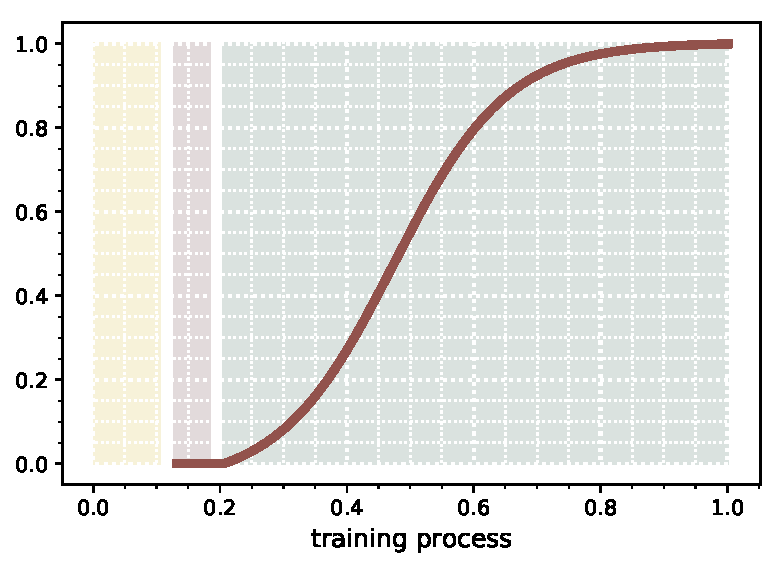
\includegraphics[width=0.4\textwidth]{contents/figures/pdf/analysis/TransferabilityOffset.pdf}
    } 
    \\
    \hspace{0mm}
    \subfloat{
        
\includegraphics[width=0.32\textwidth]{contents/figures/pdf/analysis/annotation.pdf}
        } 
    \caption{
        The changing of $\gamma$ with $\gamma_0=1$. 
        We use three different color to denote three different training stage $N_0, N_1$ and $N_2$. 
        In particular, $N_0$ is the pretrain stage on the source domain, thus $\sigma$ is not used. 
        In the stage of $N_1$, $\gamma$ is set to be $0$ so as to select most transferable samples. 
        In stage $N_2$, the $\gamma$ progressively grows according to $\sigma(\cdot)$.
    }
    \label{figure: offset changing}
\end{figure}

\subsubsection{Baseline Methods}

% Please add the following required packages to your document preamble:
% \usepackage{multirow}

% \newcommand\iw{0.0}
% \newcommand\cw{0.05}

\begin{table*}[!t]
    \renewcommand{\arraystretch}{1.3}
    \caption{Accuracy (\%) of each method with 20 and 40 shared class on Office-Home. }
    \label{table: exp on OfficeHome}
    \small
    \centering
    \begin{tabularx}{0.95\textwidth}{r Y Y Y Y Y Y Y Y Y Y Y Y >{\itshape}Y }
        \toprule[0.8pt]
        \multicolumn{1}{c}{\multirow{2}{*}{Method}} & \multicolumn{13}{c}{All Class Accuracy(\textbf{OS}) on Office-Home}                                                                                                                                                                                     \\
        \cmidrule[0.1pt]{2-14}
        \multicolumn{1}{c}{}                        & Ar$\to$Cl                                            & Ar$\to$Pr    & Ar$\to$Rw    & Cl$\to$Ar    & Cl$\to$Pr    & Cl$\to$Rw    & Pr$\to$Ar    & Pr$\to$Cl    & Pr$\to$Rw    & Rw$\to$Al    & Rw$\to$Cl    & Rw$\to$Pr    & Avg          \\

        \hline
        \multicolumn{14}{c}{\textit{results with 20 shared classes}}                                                                                                                                                                                                                                                                                                                                                         \\
        \hline
        OSVM \methodyear{[ECCV, 2014]}                                        & 32.9                                                 & 30.1         & 42.2         & 35.6         & 29.9         & 38.7         & 37.8         & 31.6         & 41.9         & 39.3         & 33.4         & 40.5         & 36.1         \\
        MMD \methodyear{[NIPS, 2007]}                                    & 28.5                                                 & 26.2         & 33.6         & 35.9         & 28.1         & 30.3         & 30.5         & 26.7         & 37.8         & 47.0         & 31.3         & 38.2         & 32.8         \\
        GRL  \methodyear{[JMLR, 2016]}                                  & 23.5                                                 & 25.7         & 31.1         & 30.4         & 31.3         & 26.9         & 27.4         & 19.8         & 35.6         & 33.5         & 28.4         & 31.9         & 28.7         \\
        ATI-$\lambda$ \methodyear{[ICCV, 2017]}                        & 48.1                                                 & 49.2         & 55.7         & 44.8         & 52.1         & 59.4         & 43.7         & 41.6         & 60.9         & 43.4         & 45.1         & 57.9         & 50.1         \\
        OSBP \methodyear{[ECCV, 2018]} & 53.1& 55.6& 62.7& 50.7& 58.5& 63& 50.5& 48.1& 63.3& 54.2& 51.7& 62.8&56.1\\

        \hline
        ThDAN-dy &54.3&56.1&64.8&51.6&59.7&63.1&54.6&55.0&63.2&57.4&53.9&66.1&58.6\\

        ThDAN & \emmax{59.8}& \emmax{61.4}& \emmax{68.4}& \emmax{56.7}& \emmax{61.7}& \emmax{67.8}& \emmax{56.0}& \emmax{57.6}& \emmax{67.8}& \emmax{58.9}& \emmax{59.5}& \emmax{68.6}& \emmax{62.0} \\
        \hline
        \multicolumn{14}{c}{\textit{results with 40 shared classes}}                                                                                                                                                                                                                                                                                                                                                         \\
        \hline
        OSBP \methodyear{[ECCV, 2018]} & 44.2& 46.3& 51.0& 41.8& 47.5& 51.9& 42.4& 40.7& 51.1& 44.4& 42.8& 52.2&46.3\\

        \hline
        ThDAN-dy &48.7&49.2&52.6&43.0&55.1&52.0&45.3&43.7&51.6&45.8&46.0&53.4&48.8\\

        ThDAN & \emmax{50.1}& \emmax{51.8}& \emmax{59.4}& \emmax{47.2}& \emmax{52.3}& \emmax{56.2}& \emmax{49.5}& \emmax{45.1}& \emmax{58.9}& \emmax{47.3}& \emmax{50.3}& \emmax{60.6}& \emmax{52.4} \\
        
        \bottomrule[0.8pt]
    \end{tabularx}
\end{table*}









We implement several baseline for comparison in this paper. (\textbf{1}) \textit{Open Set SVM \textbf{(OSVM)}} proposed in \cite{OSVM}, which utilizes the threshold probability to reject samples as unknown if the predicted probability is lower than the threshold for any class. 
% We train a feature generator on the source domain, then use OSVM to classify the features.
% Therefore, we train OSVM only using source samples and tested them on the target samples.
Addition to that, we also implement two baseline methods for close set domain adaptation in this work: 
(\textbf{2}) A combination of \textit{Maximum Mean Discrepancy \textbf{(MMD)}} based training method \cite{DeepAdaptationNetworks} and the OSVM. The MMD can be used to match the distribution between different domains for unsupervised domain adaptation. We trained the classifier networks to minimize the MMD so as to obtained domain-invariant features for training OSVM. 
(\textbf{3}) A combination of \textit{Gradient Reversal Layer \textbf{(GRL)}} \cite{DomainAdversrialNetwork} and OSVM. The GRL is widely used in domain adversarial training to match distributions across domains. Likewise, we first trained a feature generator by utilizing GRL and then train an OSVM to classify the generated features. 
Finally, we compared our method with the state-of-the-art open set domain adaptation models: 
(\textbf{4}) \textit{Assign-and-Transform-Iteratively \textbf{(ATI)}} proposed by \cite{OpensetsDA}, which is developed for the case that unknown samples in the source domain are available. Nevertheless, they applied this method using OSVM when the unknown samples are absent in the source domain. Furthermore, we show the results which utilized the unknown source samples during training, the results are cited from \cite{OpensetsDA} so as to better understand the performance of our method.
(\textbf{5}) \textit{Open Set Back-Propagation \textbf{(OSBP)}} model \cite{OpensetDA-bp} for the open set setting followed by this paper. The OSBP trains a domain adversarial network to output a class-sensitive probability which for target samples so as to  reweight the importance of target samples from the unknown classes. The class-sensitive probability is set to be $0.5$ in this paper. 
The baseline methods mentioned above build upon the same network architecture.


\subsubsection{Implementation Details}


Our model is implemented in PyTorch\footnote{https://pytorch.org/}, and adopts a pretrained AlexNet \cite{AlexNet} as a backbone network. 
In order to make a fair comparison, we follow the settings in \cite{OpensetDA-bp} to fix the parameters of the backbone networks, then constructed fully-connected layers with 100 hidden units after the $FC8$ layers and activated by Leakly-ReLU. 
Batch Normalization \cite{BatchNorm} was employed for stable training. 
We used momentum stochastic gradient descent with momentum scaler $0.9$. 
Following the practice of DANN \cite{DomainAdversrialNetwork}, the learning rate is adjusted during the training with $\mu_p=\mu_0/(1+\alpha_1\cdot p)^\alpha_2$, where $p$ is the training progress linearly changing from $0$ to $1$ ,$\mu_0=1.0 \times 10^{-3}$, $\alpha_1=10$, $\alpha_2$=0.75.
In all experiments, the $\gamma_0$ was set to be 0.1, and a scaled and shifted sigmoid function was applied for $\sigma(\cdot)$ as shown in \figurename{\ref{figure: offset changing}}. 

% Please add the following required packages to your document preamble:
% \usepackage{multirow}

% \newcommand\iw{0.05}
% \newcommand\cw{0.05}
% \renewcommand\tabularxcolumn[1]{m{#1}}
\newcommand\emmax[1]{\textcolor{red}{\textbf{#1}}}
\newcommand\methodyear[1]{\textcolor{blue}{#1}}
\newcommand\Tstrut{\rule{0pt}{2.6ex}}
\newcommand\Bstrut{\rule[-0.9ex]{0pt}{0pt}}

\begin{table*}[htb]
    \renewcommand{\arraystretch}{1.3}
    \caption{Accuracy (\%) of each method with 6 shared class on VisDA. }
    \label{table: exp on visDA}
    \centering
    \small
    \begin{tabularx}{0.95\textwidth}{r Y Y Y Y Y Y Y >{\itshape}Y >{\itshape}Y }
        \toprule[0.8pt]
        \multicolumn{1}{c}{\multirow{2}{*}{Method}} & \multicolumn{9}{c}{  class-wise accuracy on VisDA}                                                                       \\ \cmidrule[0.1pt]{2-10}
        \multicolumn{1}{c}{}                        & Bcycle                                             & Bus  & Car  & Mcycle & Train & Truck & Unkown & Avg.All & Avg.Known \\
        \hline
        OSVM  \methodyear{[ECCV, 2014]}                                      & 4.8                                                & 45.0 & 44.2 & 43.5   & 59.0  & 10.5  & 57.4   & 37.8    & 34.5      \\
        MMD  \methodyear{[NIPS, 2007]}                                  & 0.2                                                & 30.9 & 49.1 & 54.8   & 56.1  & 8.1   & 61.3   & 37.2    & 33.2      \\
        GRL  \methodyear{[JMLR, 2016]}                                   & 9.1                                                & 50.5 & 53.9 & 79.8   & 69.0  & 8.1   & 42.5   & 44.7    & 45.1      \\
        OSBP  \methodyear{[ECCV, 2018]}                                       & 48.0                                               & 67.4 & 39.2 & 80.2   & 69.4  & \emmax{24.9}  & 80.3   & 58.5    & 54.8      \\
        \hline
        ThDAN-dy                                    & 52.6                                               & 69.5 & 58.8 & 83.1   & 72.3  & 12.3  & 84.5   & 61.8    & 58.1      \\
        ThDAN                                 & \emmax{55.2}                                               & \emmax{70.8} & \emmax{61.4} & \emmax{85.6}   & \emmax{74.8}  & 10.0  & \emmax{88.8}   & \emmax{63.8}    & \emmax{59.6}      \\
        \bottomrule[0.8pt]
    \end{tabularx}
\end{table*}


\begin{figure*}[hbt!]
    \centering
    \subfloat[AlexNet Feature]{
        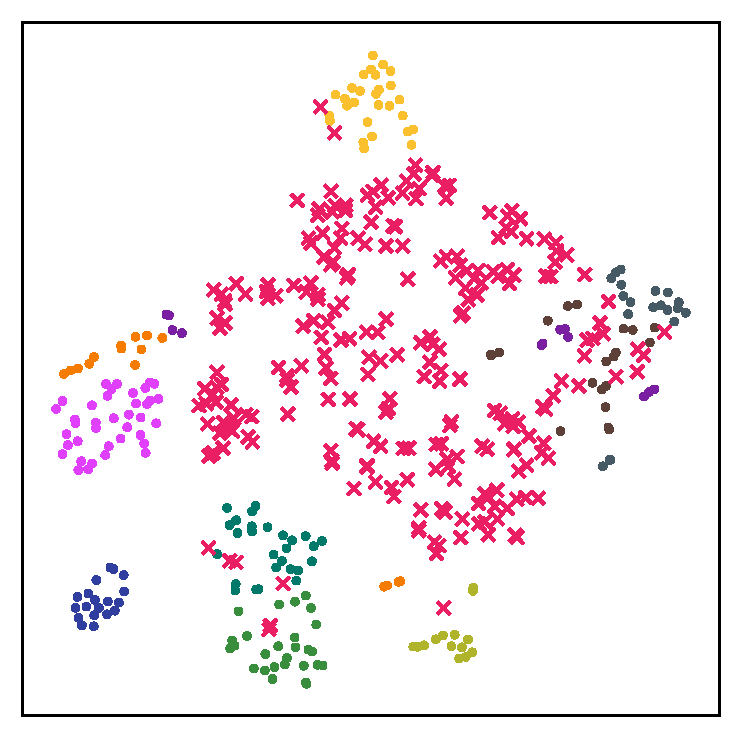
\includegraphics[width=0.235\textwidth]{contents/figures/pdf/tsne/Source.pdf} 
        \label{figure: tSNE source}
    } 
    % \hfil
    \subfloat[GRL Feature]{
        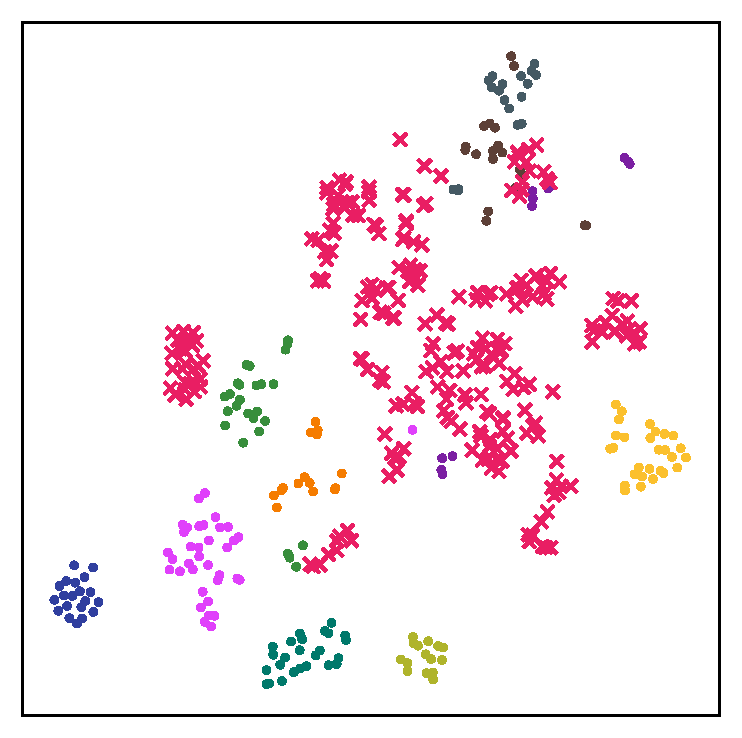
\includegraphics[width=0.235\textwidth]{contents/figures/pdf/tsne/DANN.pdf} 
        \label{figure: tSNE RGL}
    }
    % \hfil
    \subfloat[OSBP Feature]{
        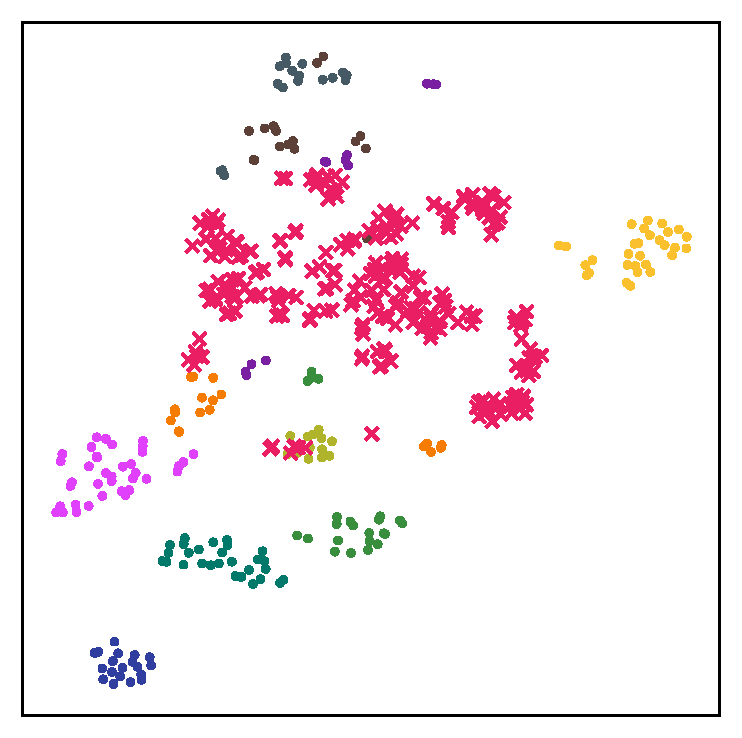
\includegraphics[width=0.235\textwidth]{contents/figures/pdf/tsne/OSBP.pdf} 
        \label{figure: tSNE OSBP}
    }
    % \hfil
    \subfloat[ThDAN Feature]{
        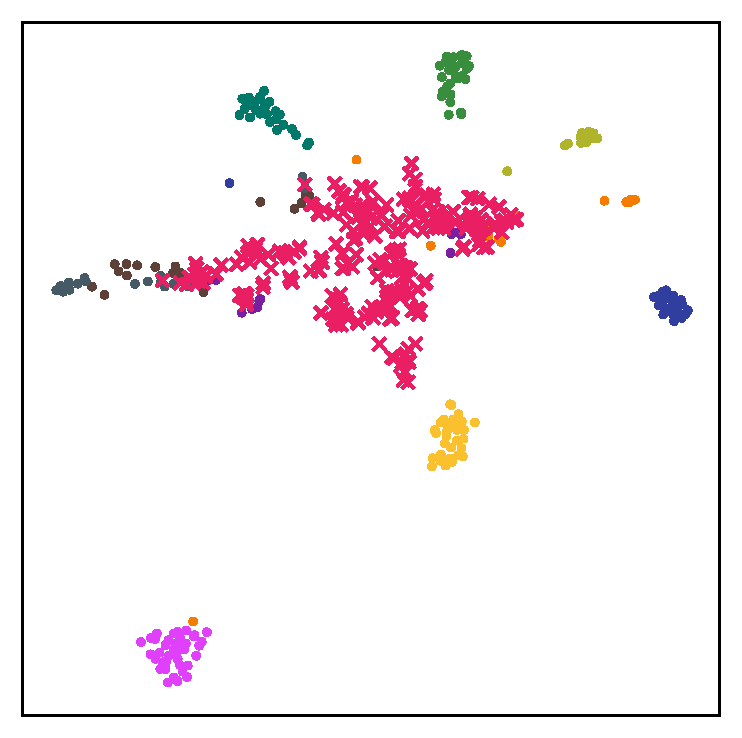
\includegraphics[width=0.235\textwidth]{contents/figures/pdf/tsne/ThDAN.pdf} 
        \label{figure: tSNE ThDAN}
    }
    \caption{
        The t-SNE visualization of obtained target features. The red cross '\unknowncolor{\textbf{$\scriptstyle\times$}}' indicate the unknown target examples, and porint of different colors indicate different known class. 
        (\textbf{a}): Feature obtained by AlexNet trained on the source domain. 
        (\textbf{b}): Features obtained by a model trained with Gradient Reversal Layer. 
        (\textbf{c}): Features obtained by OSBP. 
        (\textbf{d}): Features obtained by our model.
    } \label{figure: tSNE}
\end{figure*}



\subsection{Classification Results}

Table \ref{table: exp on office31}, \ref{table: exp on OfficeHome} and \ref{table: exp on visDA} show the classification results on the six tasks of \textbf{Office-31}, twelve tasks of \textbf{Office-Home} and one task on \textbf{VisDA}. 
The \textbf{OS} stands for accuracy of all classes, and \textbf{OS*} stands for accuracy of known classes. 
ThDAN outperforms all other methods in average accuracy on different datasets. 


\subsubsection{Result on Office-31}
The classification result on Office-31 is shown in Table\ref{table: exp on office31}. 
We use the first 10 classes as the known class and select images of these 10 categories in each domain of Office-31 as target domains. The 21-31 classes are used as unknown classes in the target domain. 
In additionally, in alphabetical order, the 11-20 classes are used as unknown samples in the source domain, which will be used for compared method ATI. 

In this part, we conduct experiments on Office-31 with three different settings,
(\textbf{1}) The CSDA setting, where the source and the target domain share the same label space.
(\textbf{2}) The OSDA of \cite{OpensetsDA}, where a partition of unknown source samples is needed to train the model.
(\textbf{3}) The OSDA we followed, where the label space of target domain subsumes the label space of source domain.

We notice that when applying methods for close set domain adaptation to open set setting, the model performance will incur a grave decay. 
That is because the models proposed for CSDA are not capable of handling the target samples from the unknown classes in OSDA setting.
We also compare with ATI model that proposed for OSDA setting which demands unknown source samples for training \cite{OpensetDA-bp}. 
When we implement ATI in the OSDA setting that we followed \cite{OpensetDA-bp}, we can notice an obvious performance drop.
This indicating the OSDA setting we followed not only more practical but also more challenging.
Comparing to the state-of-the-art OSBP model, our model can achieve plausible results in most tasks and on the average.

% In particular, ThDAN-m-dy can outperform OSDA by a reasonable margin, and even models that follows the open set setting where the unknown source samples are available. 
% Also referring to the result of Table\ref{table: exp on office31} and Table\ref{table: exp on visDA}, we conduct ablation study with different settings of ThDAN, it turns out each key component of ThDAN can improve the model performance. 



\subsubsection{Result on Office-Home}
Office-Home is a more challenge dataset for adaptation task. In alphabet order, the 40-65 classes are used as unknown samples in the target domain. And we conduct experiments with two different settings,
(\textbf{1}) The first 20 classes are used as the common label set.
(\textbf{2}) The first 40 classes are used as the common label set.

The classification result on Office-Home is shown in Table\ref{table: exp on OfficeHome}. 
As we increase the number of known classes, all models will incur performance drop. 
That is because it's harder to categorize samples from the diverse known classes than reject samples as the one unknown class.  
The proposed ThDAN can exceed the baseline OSBP in all tasks. 
Even if we double the number of known classes to make the adaptation task more difficult, ThDAN can remain superiority compared with other method.
The results in Office-Home verified the effectiveness of our method when the number of known classes varying. 

\subsubsection{Result on VisDA}
In the experiments of VisDA, the training split is used as the source domain and validation one as the target domain. 
We choose 6 categories, \textit{i.e.,} bicycle, bus, car, motorcycle, train and truck as the known classes, and the other 6 categories as the unknown classes. 
Table \ref{table: exp on visDA} shows the classification results, where \textit{Avg. All} and \textit{Avg.Known} indicate the accuracy averaged over all classes and known classes. 
For classification of known classes, ThDAN could exceeds other methods in almost every classes and in the average, which means our method can effetely transfer knowledge to the known classes. 
Also, our model improves the classification accuracy for Unknown classes by a big margin. 
This states that our method can perform well on both labeling the samples from the unknown classes and classifying the samples from the unknown classes. 

\begin{figure*}[!t]
    \centering
    \subfloat[Accuracy Comparison]{
        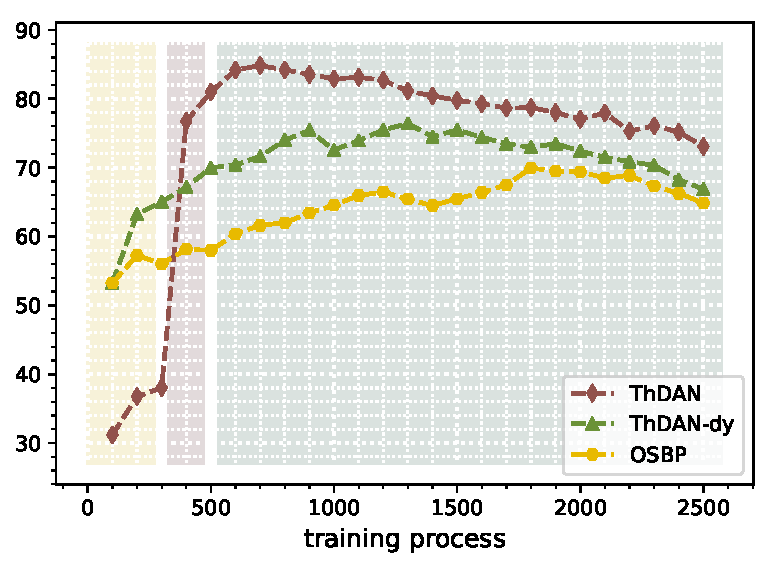
\includegraphics[width=0.33\textwidth]{contents/figures/pdf/analysis/Compare.pdf} 
        \label{figure: compares}
    } 
    \subfloat[OS and OS* Comparison]{
        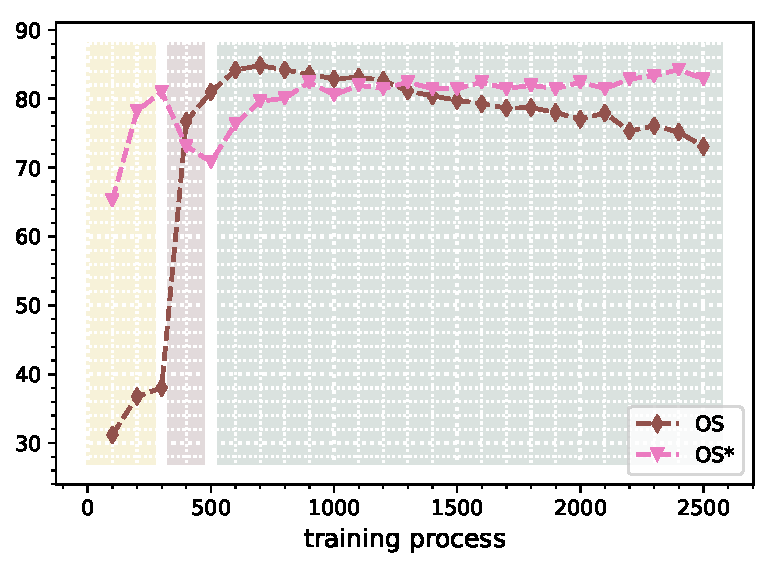
\includegraphics[width=0.33\textwidth]{contents/figures/pdf/analysis/OS.pdf} 
        \label{figure: OS and OS*}
    }
    \subfloat[Selection Accuracy]{
        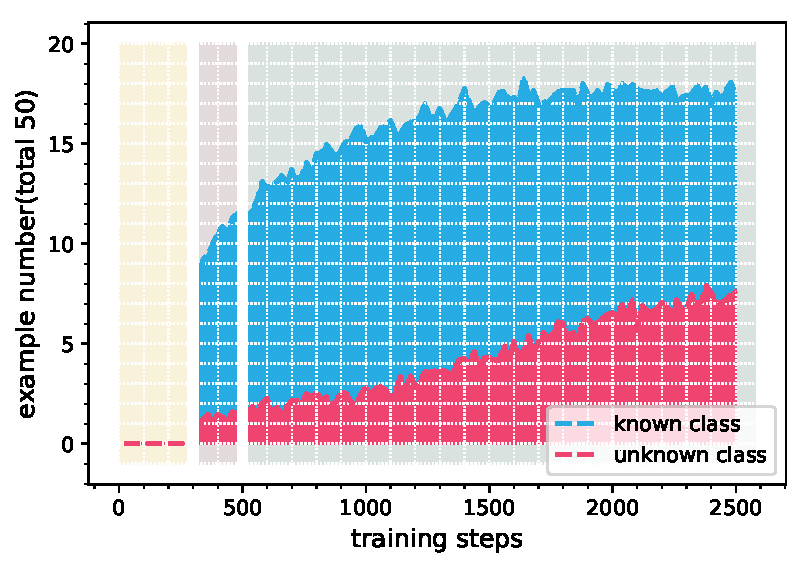
\includegraphics[width=0.33\textwidth]{contents/figures/pdf/analysis/Selection.pdf} 
        \label{figure: example selection record}
    }
    \\
    \hspace{0mm}
    \subfloat{
        
\includegraphics[width=0.32\textwidth]{contents/figures/pdf/analysis/annotation.pdf}
        } 
    \caption{
        Empirical analysis of ThDAN, we use three different color to denote different training stage as \figurename{\ref{figure: offset changing}} dose.
        (\textbf{a}): The comparison of accuracy between our model and OSBP. 
        (\textbf{b}): The \textit{All Class Accuracy \textbf{OS}} and \textit{Known Class Accuracy \textbf{OS*}}  of ThDAN during training.
        (\textbf{c}): The number of correctly selection and false selection during training. 
    }
    \label{figure: analysis}
\end{figure*}
\begin{figure}[H]
    \centering
    \subfloat[\footnotesize Accury \textit{w.r.t.} ratio of used unknown samples]{
        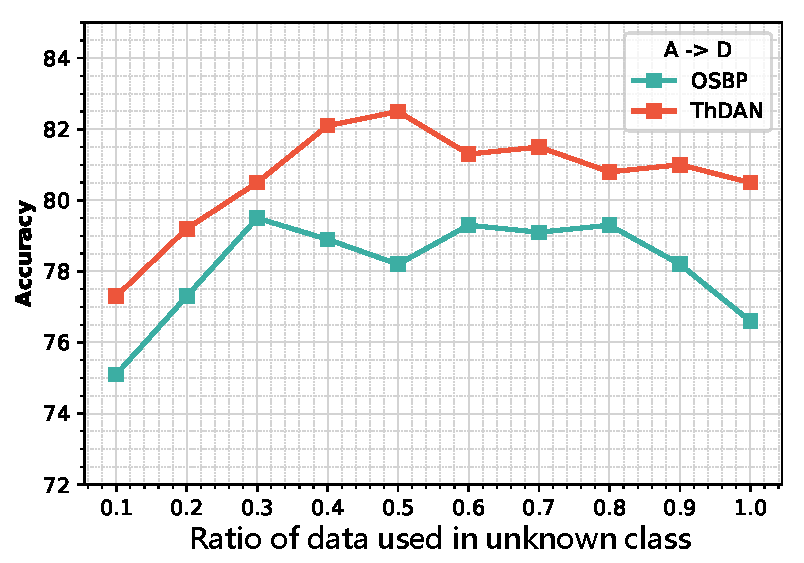
\includegraphics[width=0.34\textwidth]{contents/figures/pdf/analysis/nuknown_change.pdf} 
        \label{figure: ration of unknown}
    } 
    \subfloat[\footnotesize Accury \textit{w.r.t.} number of classes that are treated as the unknown]{
        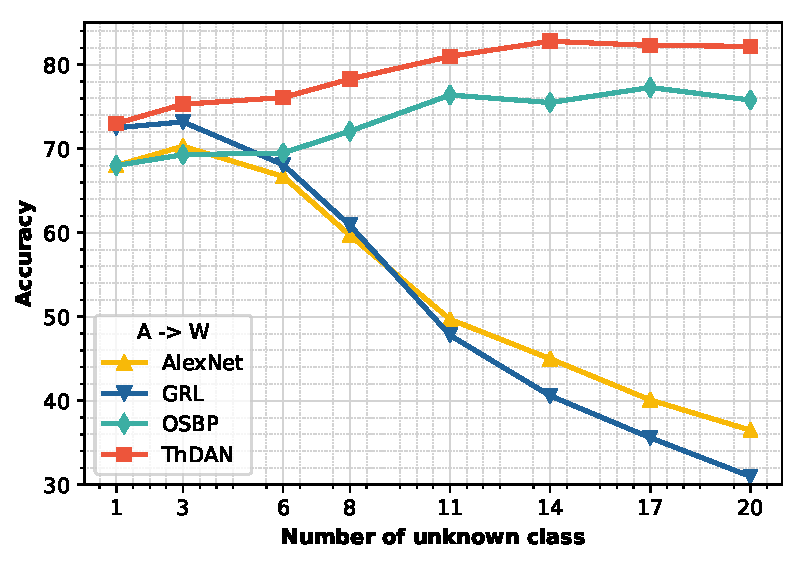
\includegraphics[width=0.33\textwidth]{contents/figures/pdf/analysis/class_change.pdf} 
        \label{figure: number of unknown class}
    }
    \subfloat[Accury \textit{w.r.t.} value of $\gamma_0$]{
        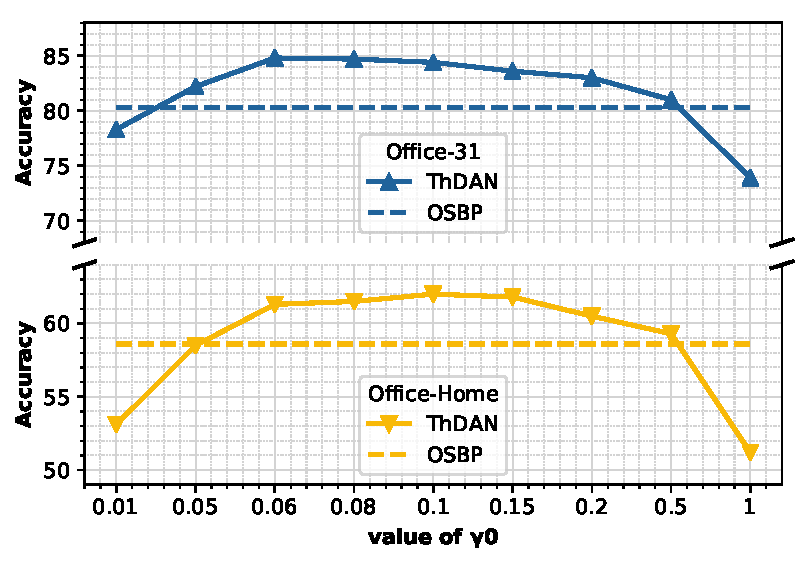
\includegraphics[width=0.33\textwidth]{contents/figures/pdf/analysis/sigma_change.pdf} 
        \label{figure: changing of sigma}
    }
    \\
    \caption{ }
    \label{figure: analysis}
\end{figure}
\subsection{Analysis}
This section conducts empirical experiments to further verify and analyse the efficiency of the proposed ThDAN.
\subsubsection{Ablation Study}
We perform an ablation study to evaluate the efficacy of the proposed threshold adjusting techniques proposed in Section\ref{Section : Progressive Sample Selection}. 
Ablation studies on Office-31, OfficeHome and VisDA datasets involve 3 kinds of ThDAN variants.
(\textbf{1}) \textit{\textbf{ThDAN-m-dy}} is the original setting driven by Equation \ref{eq: transferability thresholded}, which calculates transferability threshold based on mini-batch samples and a fixed $\gamma_0$. 
(\textbf{1}) \textit{\textbf{ThDAN-dy}} is the variant applies momentum to generate transferability threshold according to Equation \ref{eq: momentum transferability baseline}. 
And  (\textbf{1}) \textit{\textbf{ThDAN}} further takes advantage of dynamic $\gamma$ based on Equation \ref{eq: dynamic tolerable range} to calculate transferability threshold. 

The bottom rows of Table \ref{table: exp on office31}, \ref{table: exp on OfficeHome} and \ref{table: exp on visDA} show the results.
The most direct observation is that the techniques applied to adjust the threshold will substantially affect the final results, which indicates the transferability threshold is important to the ThDAN.
We notice ThDAN-m-dy is comparable to the baseline model OSBP, meaning that the sample selection strategy works for OSDA. 
ThDAN-dy outperforms ThDAN-m-dy, which shows the momentum transferability threshold of Equation\ref{eq: momentum transferability baseline} can deliver a more solid threshold. 
ThDAN exceeds both ThDAN-m-dy and ThDAN-dy in most tasks, indicating the dynamic $\gamma$ of on Equation \ref{eq: dynamic tolerable range} is also substantial to the model performance.


\subsubsection{Feature Visualization}
To verbify the proposed model can produce distinguishable features for the samples from the known classes and separable features for the samples from the unknown classes, we visualize the t-SNE embeddings of the bottleneck representations of the target samples in \figurename{\ref{figure: tSNE}}.
We compare the ThDAN with AlexNet that trained on the source domain, GRL that proposed for CSDA and OSBP that proposed for OSDA. 
The experiment is conducted on the adaptation task \textbf{$A10\to W20 $}.
\figurename{\ref{figure: tSNE source}} shows that the initial features before adaptation. 
\figurename{\ref{figure: tSNE RGL}} presents the features obtained by GRL. 
The features are mixed together, meaning that it is difficult for GRL to distinguish samples from known and unknown classes. 
\figurename{\ref{figure: tSNE OSBP}} shows that OSBP can produce more discriminate features for the unknown class than GRL. 
\figurename{\ref{figure: tSNE ThDAN}} shows the features generated by ThDAN, it is obvious that our model can produce features that are more discriminating than other models. 
We can notice the feature cluster of OSBP and ThDAN are more separable comparable with the method proposed for OSDA. 
This 
The feature cluster of the unknown class is tighter than other methods, and the feature clusters of the known classes are more distinguishable. 


\subsubsection{Convergence Performance}
\figurename{\ref{figure: compares}} compares the converge performance of our model and OSBP. 
We can observe that the ThDAN-m can deliver the optimal point more rapidly. 
Since ThDAN requires pretraining on the source domain, the accuracy in the early stage is quite low. 
However, when ThDAN-dy starts domain adversarial training in the stage $N_1$, accuracy increases rapidly and exceeds the performance of OSBP about 10 percents, which demonstrates the effectiveness of the sample selection strategy. 

In order to have a more detailed understanding of ThDAN, we illustrates the \textit{All Class Accuracy (OS)} and \textit{Known Class Accuracy (OS*)} during training in \figurename{\ref{figure: OS and OS*}}. 
In the pretraining stage $N_0$, the model can only learn from the source domain, so it completely incapable of categorizing unknown class data, which leads to the lowness of OS*. 
In the stage $N_1$, the OS will temporarily decrease and OS* will boost, for the reason that the model will reject most samples as 'unknown'. 
In the last stage $N_2$, as the $\gamma$ increases progressively, more target samples from the known classes will be selected for domain adversarial training. As a result, the accuracy of OS* gradually increases, and meets the accuracy of OS at a point. 

\subsubsection{Varing the Number of Unknown Samples and Number of Unknown Classes}
The sampling proportion between the data from known and unknown classes can substantially affect the model performance.
However, in real scenarios, can not manually set the sampling proportion due to the lack of target label information.
During the training phase, ThDAN is confined to randomly sample training data from the target domain.
Therefore we conduct experiments to implicitly change the sampling proportion by varying the number of unknown data and the number of unknown classes.
All experiments are conducted on Office-31 datasets.

We first fix the number of unknown classes to 10, and then change the sample number of each unknown class.
The ratio 0.1 of sample number indicates that only one-tenth samples of each unknown class are used for training and testing, while the others are discarded from the dataset.
\figurename{\ref{figure: ration of unknown}} shows the result.
When the ratio is low, the model can hardly identify samples from unknown classes for the lack of training samples. 
On the contrary, when the ratio is high, the negative transfer of unknown class would undermine the classification of known classes. 
Thus, the performance of model is defective around the end point of the interval. 

We further vary the number of unknown classes in \figurename{\ref{figure: number of unknown class}}.
As the number of unknown classes increases, the performance of methods for CSDA will decrease significantly. 
That is because they cannot alleviate the negative transfer brought by the unknown classes, which stresses the importance of developing methods for the open set domain adaptation. 
The model proposed for OSDA would gains performance improvement by correctly rejecting samples from unknown classes. 
That is because it's easier to reject samples as the one unknown class than categorize samples from the diverse known classes.  
The accuracy has the trend to decay due to that too many unknown classes would interfere with the model performance on classification.


\subsubsection{Sample Selection Accuracy}
This subsection analyzes the behavior of sample selection algorithm by inspecting the selection accuracy. 
We record the number of samples that are selected for domain adversarial training, and illustrates the correct selection (selecting the target samples from the known classes) and the false selection for a batch of size 50 samples in \figurename{\ref{figure: example selection record}}. 
Then we can make observations from different stages. 
In $N_1$, the selection algorithm can filter out most target samples from the unknown classes. In particular, for a batch consisted of about 25 unknown class examples, only about 2 unknown class examples are selected for domain adversarial training. Although the $\gamma$ remains to 0 in $N_1$, we can notice an obvious growth in the number of correct selection, which means that our model can accept more the known class examples by learning from high transferable examples. 
In stage $N_2$, as the $\gamma$ gradually tweaked, more samples are selected by the algorithm, both the correct and false selection increases. And it is obvious that in the early stage of $N_2$, the number of correct selection grows faster than the number of false selection, which demonstrates the efficiency of the Progressive Sample Selection strategy. Note that our model delivers the optimal solution in this stage. 

\subsubsection{Change in Upper Bound of Transferability Offset}
We analyze the behavior of our model when the $\gamma_0$ changes, since it is an important hyperparameter that we need to set. 
As is shown in \figurename{\ref{figure: changing of sigma}}, the upper $\gamma$ has a significant impact on the result, a very low value of $\gamma_0$ implies that the model can only align with a small batch of transferable target samples, thus the ThDAN can not outperform the OSBP. 
On the other hand, a very high value of $\gamma_0$ will allow the model to select more samples from the unknown classes for domain adversarial training, resulting in poor performance. 

Our model can deliver plausible result on both Office-31 and Office-Home datasets when the $\gamma_0$ in the range of $[0.06, 0.5]$, which indicates that our model is insensitive to the setting of $\gamma_0$. 
That is because when we gradually increase the $\gamma$ during training, we also gradually decrease the learning rate. 
As a result, the transferable samples that selected in early stage would ‘dominate’ model training, because they engage in training sooner, and the gradient produced by them can update model with greater learning rate. 
As the $\gamma$ approaches $\gamma_0$, the learning rate is relatively small, and the previously selected samples would still be selected for training, thus the newcomer has little impact for model performance. 
This directly reflect on the insensitivity of value of $\gamma_0$ to the accuracy of training. 


